\chapter{TINJAUAN PUSTAKA}
\vspace{1ex}

\section{\textit{State of the Art}}
\begin{enumerate}
	\item Lightweight Residual Network for Person Re-Identification (Reza Fuad Rachmadi, Supeno Mardi Nugroho, I Ketut Eddy Purnama) \cite{cit:14}
	\par
	\textit{Lightweight Residual Network for Person Re-Identification} ini merupakan sebuah implementasi \textit{lightweight CNN} untuk melakukan re-Identifikasi manusia, lightweight CNN yang digunakan berbasis \textit{Residual Network} dengan menggunakan pre trained weights yang pernah  digunakan untuk memecahkan masalah klasifikasi CIFAR-10. Berdasarkan hasil dari riset yang dilakukan, meskipun lightweight CNN tidak mendapatkan akurasi tercanggih dibandingkan model-model lainnya, banyak nya informasi yang didapatkan oleh model ini sangat tinggi, dan dapat dikatakan model ini lebih efisien dari model-model lainnya.
	\vspace{1ex}
	
	\item Torchreid: A Library for Deep Learning Person Re-Identification in Pytorch. (Kaiyang Zhou, Tao Xiang). \cite{cit:16}
	\par
	Torchreid merupakan sebuah \textit{library deep learning} yang dibuat oleh Kaiyang Zhou untuk mempercepat implementasi dan percobaan re-identifikasi. Library ini secara umum dibuat dengan menggunakan bahasa Python dengan beberapa kode berbasis Cython untuk optimisasi. Pada library ini dataset sudah di \textit{preprocess} dan di implementasi sesuai dengan protokol evaluasi masing masing dataset sehingga dapat dibandingkan dengan penelitian lain yang terkait.
	\vspace{1ex}
	
	\pagebreak
	
	\item Adaptive L2 Regularization in Person Re-Identification. (Xingyang Ni, Liang Fang, Heikki Huttunen) \cite{cit:17}
	\par
	
	\textit{Adaptive L2 Regularization in Person Re-Identication} merupakan sebuah penelitian untuk menambahkan regularisasi L2, dimana faktor regularisasi dapat berubah ubah secara adaptif pada \textit{baseline} model. Dari hasil penelitan yang dilakukan regularisasi L2 secara adaptif dapat meningkatkan akurasi model sekitar 1 hingga 2\% untuk \textit{dataset} Market-1501, DukeMTMC dan MSMT17.
	\vspace{1ex}
	
	\item Cross-Domain Adversarial Feature Learning for Sketch
	Re-identification. (Lu Pang, Yaowei Wang, Yi-Zhe Song, Tiejun Huang, Yonghong Tian) \cite{cit:12}
	\par
	
	\textit{Cross-Domain Adversarial Feature Learning for Sketch Re-identification} merupakan penelitian yang pertama kali menggunakan gambar sketsa sebagai input dari model re-identifikasi manusia, namun dari model yang digunakan sendiri merupakan model yang telah di optimisasi untuk melakukan pengambilan informasi dari sketsa, seperti Triplet SN dan model GN Siamese yang merupakan gabungan dari dua cabang dari model GoogleNet yang dioptimisasi dengan menggunakan pairwise verification loss.
	\vspace{1ex}
	
\end{enumerate}
\par Dapat dilihat dari penelitian-penelitian terkait diatas, selain pada penelitian \textit{Cross-Domain Adversarial Feature Learning for Sketch Re-identification}, fokus dari permasalahan adalah penggunaan metode re-identifikasi pada citra manusia yang tertangkap pada CCTV. Sedangkan pada penelitian yang kami usulkan merupakan implementasi re-identifikasi pada citra orang riil yang tertangkap pada CCTV, menggunakan citra sketsa \textit{full body} sebagai \textit{input}.
Selain itu penelitian yang dilakukan menggunakan model \textit{lightweight classical} seperti ResNet, yang bukan merupakan fokus dari penelitian \textit{Cross-Domain Adversarial Feature Learning for Sketch Re-identification}.
\vspace{1ex}

\section*{}
Demi mendukung penelitian ini, dibutuhkan beberapa teori penunjang sebagai bahan acuan dan referensi. Dengan demikian penelitian ini menjadi lebih terarah. 
\vspace{1ex}

\section{Machine Learning}
\vspace{1ex}

\begin{figure} [!htb]
	\centering
	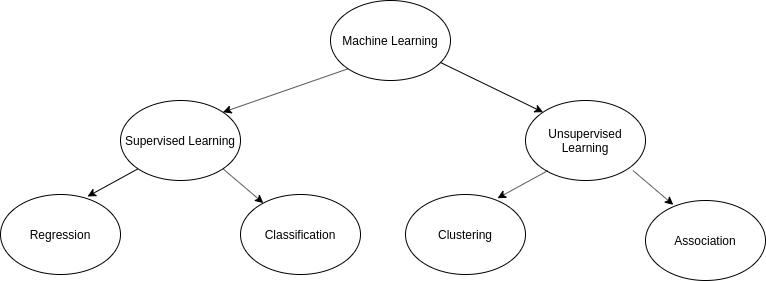
\includegraphics[scale=0.28]{img/machinelearning.png}
	\caption{Jenis Machine Learning}
	\label{fig:2.0}
\end{figure}

\textit{Machine learning} atau pembelajaran mesin adalah suatu cabang teknologi yang menerapkan penggunaan \textit{artificial intelligence}. \textit{Machine learning} pertama kali diperkenalkan oleh Thomas Bayes, Adrien-Marie Legendre, dan Andrey Markov pada sekitar tahun 1920\cite{cit:7}. Dengan berkembangnya \textit{machine learning}, tugas-tugas yang dilakukan oleh \textit{machine learning} ini pun semakin beragam, dimana secara umum jenis pembelajaran pada Machine Learning dapat dikelompokkan menjadi dua, yaitu Supervised Learning dan Unsupervised Learning.

\vspace{1ex}
\par \textit{Supervised learning} jika diartikan secara harfiah adalah pembelajaran yang ada supervisornya. Disini supervisi dilakukan oleh orang yang melakukan training kepada label di setiap datanya. Sebagai contoh dapat dilihat pada gambar \ref{fig:2.1}. 
\vspace{1ex}

\begin{figure} [!htb]
	\centering
	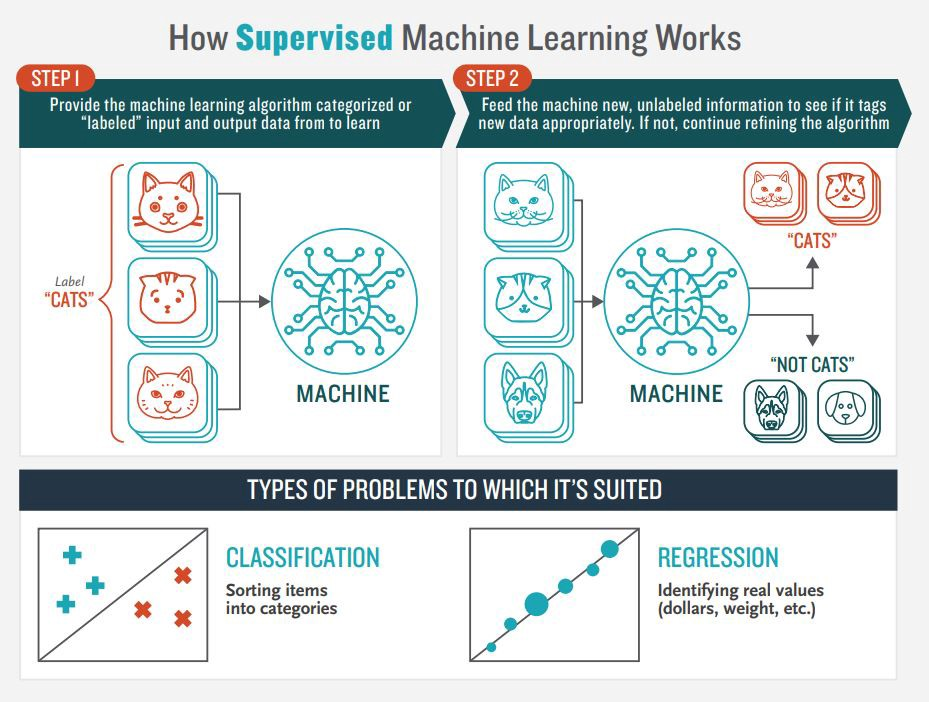
\includegraphics[scale=0.16]{img/supervised.jpeg}
	\caption{Cara Kerja Supervised Learning\cite{cit:8}}
	\label{fig:2.1}
\end{figure}

\par Pada gambar diatas, masing-masing gambar kucing diberi label “CATS” dan yang bukan kucing (“anjing”,”beruang”,”lain-lain”) diberi label “NOT CATS”. Ketika gambar baru dimasukkan setiap label akan dicompare sampai selesai, dan yang memiliki persentase lebih banyak akan diambil sebagai prediksi akhir.

\vspace{1ex}

\par Pada pendekatan \textit{supervised learning}, terdapat input dan output yang dibuat menjadi hubungan matematis. \textit{Supervised learning} cocok untuk digunakan untuk memprediksi dimana sudah ada contoh data yang lengkap, sehingga pola yang terbentuk adalah hasil pembelajaran dari data lengkap tersebut. Beberapa algoritma yang termasuk dalam \textit{supervised learning} adalah sebagai berikut:
\begin{enumerate}
	\vspace{-2mm}
	\item Regresi Linier Berganda
	\vspace{-2mm}
	\item Analisis Deret Waktu
	\vspace{-2mm}
	\item \textit{Decision Tree} dan \textit{Random Forest}
	\vspace{-2mm}
	\item \textit{Naive Bayes Classifier}
	\vspace{-2mm}
	\item \textit{Nearest Neighbor Classifier}
	\vspace{-2mm}
	\item \textit{Artificial Neural Network}
	\vspace{-1mm}
\end{enumerate}
\par Jika dibandingkan dengan \textit{supervised learning}, \textit{unsupervised learning} tidak membutuhkan adanya label sebagai dasar prediksi melainkan menggunakan kesamaan atribut - atribut yang dimiliki oleh data tersebut. Jika atribut - atribut tersebut memiliki kesamaan maka data tersebut akan di \textit{cluster} menjadi satu. Sebagai contoh dapat dilihat pada gambar \ref{fig:Unsupervised} :

\begin{figure}[h!]
	\centering
	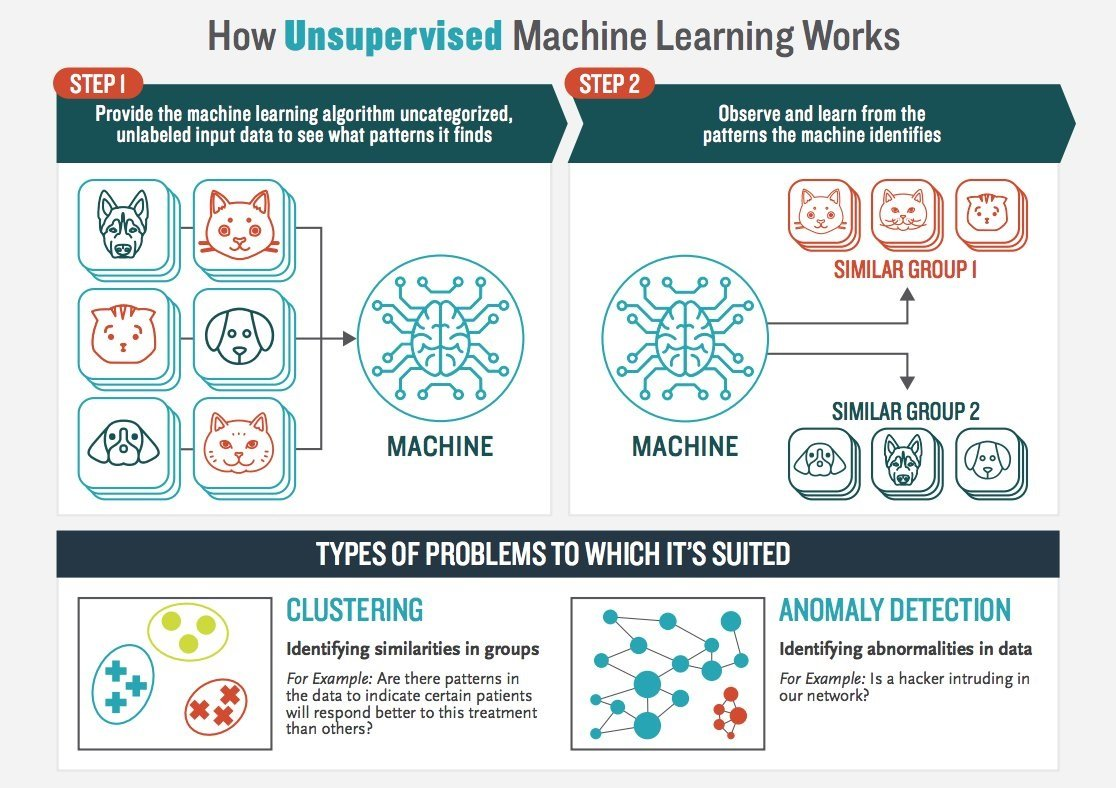
\includegraphics[scale=0.18]{img/unsupervised.jpg}
	\caption{Cara kerja Unsupervised Learning \cite{cit:8}}
	\label{fig:Unsupervised}
\end{figure}

\pagebreak

\par Pada Gambar \ref{fig:Unsupervised} dapat dilihat bahwa disediakan gambar- gambar yang tidak memiliki label ke algoritma \textit{machine learning}. Setelah itu \textit{artificial intelligence} akan memisahkan gambar mana yang memiliki kesamaan di dalam \textit{cluster}. \textit{Cluster} yang ada merupakan hasil akhir klasifikasi yang dilakukan.

\par Namun \textit{unsupervised learning} tidak memiliki hasil spesifik layaknya pada \textit{supervised learning}. Hal ini dikarenakan tidak adanya label dasar (ground truth). Beberapa algoritma yang digunakan di \textit{unsupervised learning} :
\begin{enumerate}
	\vspace{-2mm}
	\item \textit{Clustering}
	\vspace{-2mm}
	\item \textit{Anomaly Detection}
	\vspace{-2mm}
	\item \textit{Training Model}
	\vspace{-2mm}
	\item \textit{Association Discovery}
\end{enumerate}

\vspace{1ex}

\par \textit{Deep learning} (Pembelajaran Dalam) merupakan bagian yang dalam dari \textit{machine learning} yang terdiri dari pemodelan fungsi yang ditata berlapis dan mendalam dengan menggunakan \textit{Artificial Neural Network} (ANN). ANN merupakan sebuah teknik atau pendekatan pengolahan informasi yang terinspirasi oleh cara kerja sistem saraf biologis, khususnya pada sel otak manusia dalam memproses informasi. Jenis pembelajaran dalam deep learning berupa \textit{supervised, semi-supervised}, dan \textit{unsupervised}. Deep learning dapat diimplementasikan dalam pengenalan citra, pengenalan suara, klasifikasi teks, dan sebagainya.

\section{Convolutional Neural Network}
\vspace{1ex}

\begin{figure}[h!]
	\centering
	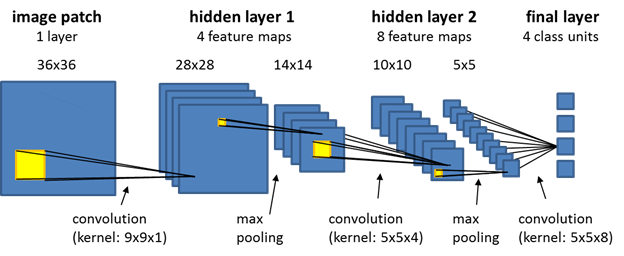
\includegraphics[scale=0.55]{img/CNN_scheme.png}
	\caption{Convolutional Neural Network}
	\label{fig:Convolutional Neural Network}
\end{figure}


Convolutional Neural Network merupakan salah satu algoritma \textit{Deep Learning} yang umum digunakan untuk data berbentuk citra. Convolutional Neural Network memiliki kedalaman yang cukup tinggi sehingga termasuk dalam jenis \textit{Deep Neural Network}. Pada umumnya CNN tidak jauh berbeda dengan neural network pada umumnya, CNN terdiri dari neuron yang memiliki \textit{weight, bias}, dan \textit{activation function}. Dimana weight dari CNN sendiri didapatkan dari persamaan sebagai berikut

\[neuron_{input} \times neuron_{output} \times tinggi \times lebar\] 

Pada Convolutional Neural Network, operasi yang paling utama merupakan Convolutional Layer, dimana terjadi operasi konvolusi pada \textit{output} dari \textit{layer} sebelumnya. Operasi konvolusi merupakan aplikasi kernel pada citra di semua offset sehingga citra secara keseluruhan diubah. Tujuan dari dilakukannya konvolusi itu sendiri adalah untuk melakukan ekstraksi dari fitur-fitur milik citra input.

\section{\textit{Triplet Loss}}
\vspace{1ex}

\begin{figure}[h!]
	\centering
	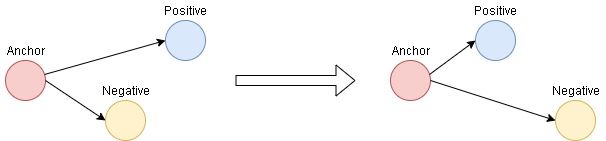
\includegraphics[scale=0.4]{img/TripletLoss.png}
	\caption{Triplet Loss}
	\label{fig:Triplet}
\end{figure}

\par \textit{Triplet Loss} merupakan sebuah \textit{Loss Function} yang umumnya digunakan dalam proses Re-Identifikasi. Pada fungsi ini dilakukan perbandingan jarak antara titik acuan terhadap titik positif yang merupakan gambar dalam kelas sama, dan perbandingan dengan titik negatif yang berasal dari kelas berbeda. Fungsi ini memastikan bahwa jarak ke titik positif akan lebih dekat dibandingkan dengan titik negatif.

\section{CycleGAN}
\vspace{1ex}

\begin{figure}  [!htb]
	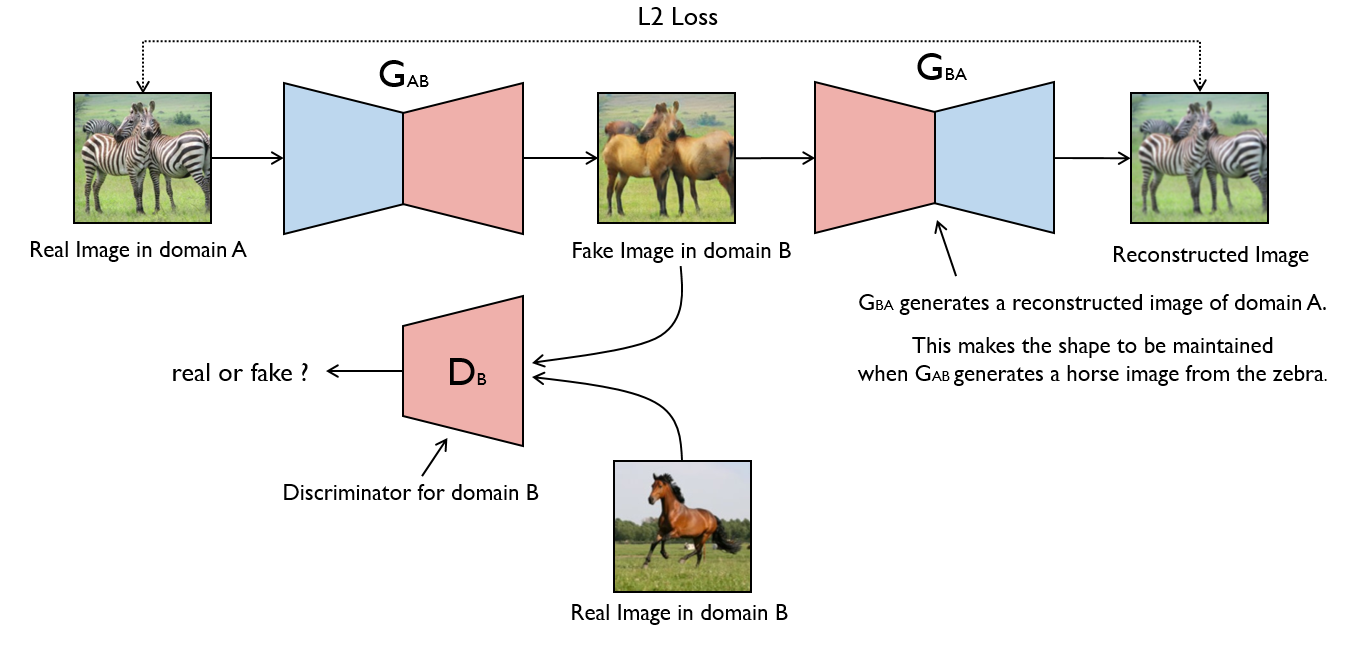
\includegraphics[scale=0.2]{img/cyclegan.png}
	%\caption{Diagram alur kerja}
	\caption{CycleGAN}
	\label{fig: 3_27}
\end{figure}

CycleGAN merupakan sebuah teknik yang menggunakan \textit{Deep Convolutional Neural Network} untuk melakukan sinstesis sebuah gambar versi baru dengan modifikasi yang diinginkan, seperti mengubah gambar dari musim panas ke musim salju. Pada umumnya \textit{training} model untuk melakukan hal tersebut membutuhkan dataset dengan contoh berpasangan(\textit{paired example}) yang sangat besar. Cara seperti ini membutuhkan waktu yang sangat lama, dan pada beberapa kasus tertentu tidak dapat dilakukan. Namun dengan menggunakan CycleGAN, model dapat secara otomatis melakukan \textit{training} untuk translasi \textit{Image-to-image}.  dilatih secara \textit{unsupervised} dengan menggunakan kumpulan gambar dari sebuah domain X ke sebuah domain Y, tanpa harus memasangkan kedua gambar tersebut.

\section{\textit{Local Binary Pattern}}
\vspace{1ex}

\begin{figure}  [!htb]
	\centering
	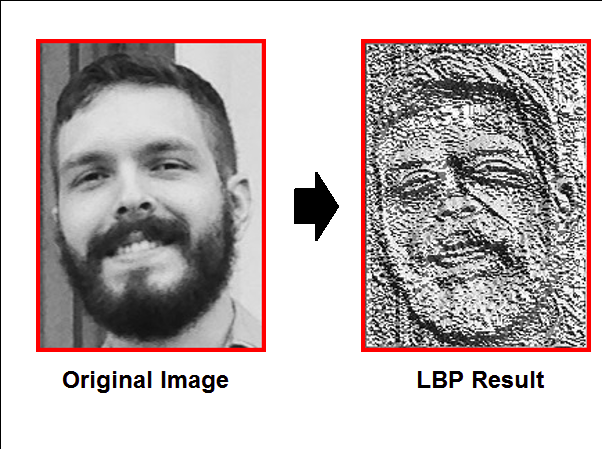
\includegraphics[scale=0.2]{img/lbp.png}
	%\caption{Diagram alur kerja}
	\caption{Local Binary Pattern}
	\label{fig: 3_27}
\end{figure}

\textit{Local Binary Pattern} (LBP) merupakan salah satu deskriptor visual yang digunakan pada visi komputer. Pada umumnya LBP digunakan pada Face Recognition dikarenakan LBP merupakan deskriptor yang sangat kuat untuk melakukan klasifikasi tekstur. Selain itu telah ditemukan bahwa ketika LBP digabungkan dengan deskriptor \textit{Histogram of Oriented Gradients} (HOG), performa yang didapatkan bertambah secara drastis pada beberapa dataset tertentu.

\par Cara kerja dari LBP sendiri adalah sebagai berikut:
\begin{enumerate}
	\vspace{-2mm}
	\item Ubah citra menjadi bentuk \textit{grayscale} / hitam putih.
	\vspace{-2mm}
	\item Bagi citra menjadi beberapa bagian(\textit{cell})
	\vspace{-2mm}
	\item Untuk setiap \textit{pixel} yang terdapat pada sebuah \textit{cell}, bandingkan dengan pixel milik 8 neighbor yang terdapat di sekelilingnya
	\vspace{-2mm}
	\item Apabila nilai dari pixel yang di tengah lebih besar dari setiap pixel pada neighbornya maka pixel tersebut diberi nilai 0, selain itu pixel tersebut diberi nilai 1.
	\vspace{-2mm}
	\item Hitung Histogram
	\vspace{-2mm}
	\item Normalisasi Histogram.
\end{enumerate}

\vspace{1ex}

\section{\textit{Fully-Connected Layer}}
\vspace{1ex}
\textit{Fully Connected layer} merupakan \textit{layer} yang bertujuan untuk melakukan transformasi pada dimensi data agar klasifikasi secara linear dapat dilakukan, dimana setiap neuron pada \textit{convolution layer} ditransformasi terlebih dahulu menjadi satu dimensi. Namun hal tersebut dapat menyebabkan hilangnya data spasial, sehingga pada umumnya fully connected layer hanya diimplementasikan pada akhir jaringan. \textit{Convolution layer} dengan ukuran kernel 1x1 dapat melakukan fungsi yang sama dengan \textit{Fully Connected Layer}, namun dapat tetap mempertahankan data spasial.
\vspace{1ex}

\section{\textit{Residual Network}}
\vspace{1ex}

\begin{figure}[h!]
	\centering
	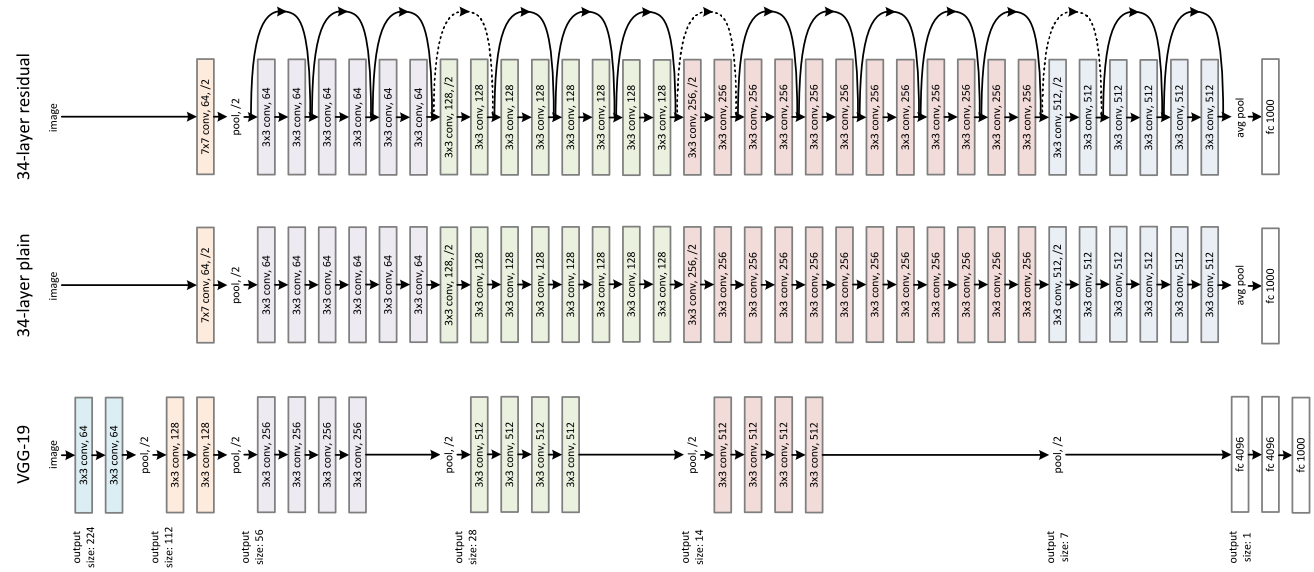
\includegraphics[scale=0.18]{img/ResNet.png}
	\caption{Perbandingan layer ResNet, plain, dan VGG-19 \cite{cit:10}}
	\label{fig:Resnet}
\end{figure}
\vspace{1ex}

\textit{Residual Neural Network} atau \textit{ResNet} merupakan sebuah \textit{Artificial Neural Network} (ANN) yang dibuat berdasarkan bentuk korteks serebral milik manusia. \textit{Residual Network} melakukan hal ini dengan memperkenalkan \textit{skip connection} atau \textit{shortcut}, dimana model dapat melompat dua atau tiga \textit{layer} jika memang hal tersebut merupakan hasil terbaik. Sebelum adanya model \textit{Residual Neural Network} penambahan layer pada suatu model hanya akan meningkatkan akurasi sampai suatu batas tertentu, sehingga penambahan layer setelah 20 hanya menambahkan kompleksitas model. Namun pada penelitian \textit{Deep Residual Learning for Image Recognition} yang dibuat oleh Kaiming He pada tahun 2015 memproposikan sebaliknya, apabila layer tambahan yang ada dapat mempelajari matriks identitas, maka akurasi minimal yang didapat pada \textit{layer} akan sama dengan apabila tidak menambahkan \textit{layer}. Untuk membuktikan hal tersebut dibuatlah sistem \textit{skip connection} atau \textit{shortcut} sehingga model dapat mempelajari matriks identitas dengan lebih mudah. Dari penelitian yang dilakukan pada dataset \textit{ImageNet}, \textit{Residual Network} dapat mengurangi \textit{loss} yang didapat ketika menambahkan lebih banyak \textit{layer} pada \textit{Artificial Neural Network} yang dibuat. \cite{cit:10}

\section{\textit{Lightweight Residual Network}}
\vspace{1ex}

\begin{figure}[h!]
	\centering
	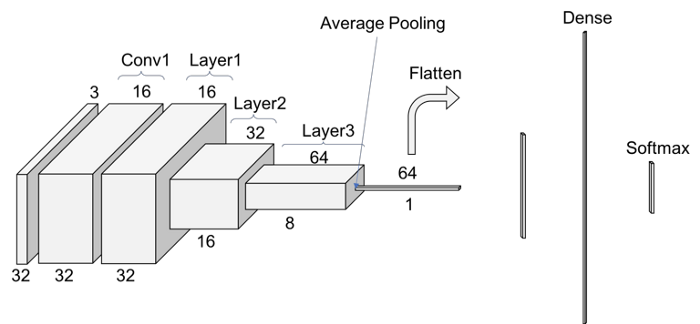
\includegraphics[scale=0.3]{img/StructureLightweightResNet.png}
	\caption{Skema struktur ResNet pada CIFAR10}
	\label{fig:ResnetScheme}
\end{figure}

Lightweight Residual Network merupakan implementasi dari Residual Network pada dataset CIFAR-10, sebuah dataset yang terdiri dari 60000 gambar 32x32, dimana setiap kelas memiliki 6000 gambar. Residual Network yang digunakan untuk memecahkan masalah klasifikasi CIFAR-10 ini berbeda dengan Residual Network pada normalnya yang memiliki jumlah parameter jauh lebih besar, yaitu sekitar 23 juta parameter. Residual Network ini memiliki jumlah layer yang relatif dalam apabila dibandingkan dengan Residual Network yang \textit{original}, namun parameter yang terdapat pada model ini jauh lebih sedikit, dengan yang paling banyak sebesar 3 juta parameter. Hal ini dikarenakan jumlah filter yang digunakan oleh model lightweight jauh lebih sedikit dibandingkan pada model konvensional, dimana pada model ResNet 50 filter yang digunakan adalah sebanyak 64 hingga 2048 filter, sedangkan pada model ResNet 56 filter yang digunakan hanyalah sebanyak 16 hingga 64 filter.

Pada gambar \ref{fig:ResnetScheme} dapat dilihat skema yang secara umum digunakan oleh Residual Network pada CIFAR10, dimana terlihat pada skema bahwa tidak terdapat \textit{pooling layer} setelah \textit{convolution layer}. Pada \textit{convolution layer} ini dapat dilihat bahwa layer pertama merupakan \textit{convolution layer} dengan ukuran 3x3 dan batch normalization. Ukuran \textit{stride} dan \textit{padding} yang diberikan adalah 1 untuk menyamakan bentuk output dengan input. Convolution Layer dari ResNet dapat dilihat dari gambar \ref{fig:Resnetconv}.

Kemudian setelah \textit{Convolution Layer}, dibuat sebuah layer yang terdiri dari 6 konvolusi dengan ukuran 3x3, banyaknya kumpulan konvolusi yang digunakan akan menentukan ukuran ResNet yang dibuat. Penurunan dimensi dari data dilakukan pada tahap ini dengan melakukan penambahan \textit{stride} menjadi dua untuk setiap konvolusi pertama di setiap layer berikut. 

\begin{figure}[h!]
	\centering
	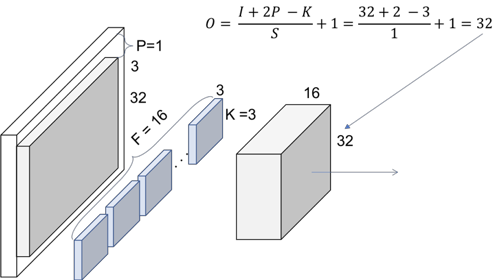
\includegraphics[scale=0.35]{img/convlightresnet.png}
	\caption{Convolution Layer Residual Network}
	\label{fig:Resnetconv}
\end{figure}

Pada layer ini diberikan \textit{bypass connection}, dimana apabila terjadi pengurangan performa dari model, dapat dilakukan \textit{bypass connection} dengan cara menambah padding dimensi dengan \textit{zeros} sehingga ukuran output sesuai dengan ukuran sebelumnya.

\begin{figure}[h!]
	\centering
	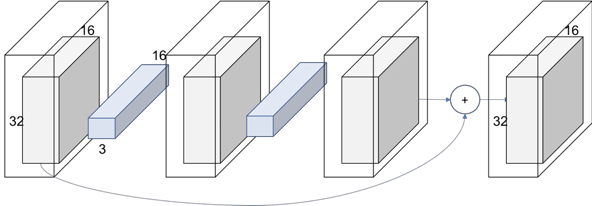
\includegraphics[scale=0.3]{img/layer1.png}
	\caption{Layer1 Residual Network}
	\label{fig:ResnetLayer1}
\end{figure}

Layer kedua memiliki cara kerja yang sama dengan layer pertama, namun dikarenakan ukuran \textit{stride} pada layer pertama dibuat menjadi dua, ukuran output adalah setengah dari input untuk layer kedua, sehingga diberikan \textit{zero padding}.

\begin{figure}[h!]
	\centering
	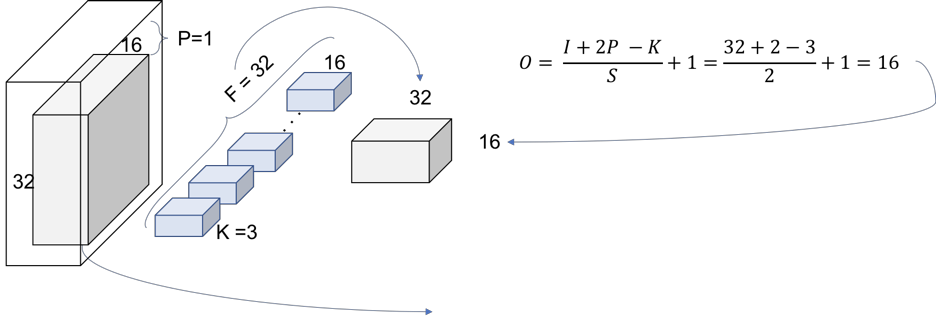
\includegraphics[scale=0.3]{img/layer2.png}
	\caption{Layer2 Residual Network}
	\label{fig:ResnetLayer2}
\end{figure}


Kemudian Layer 3 akan mengimplementasikan prinsip yang sama dengan Layer 2.

\begin{figure}[h!]
	\centering
	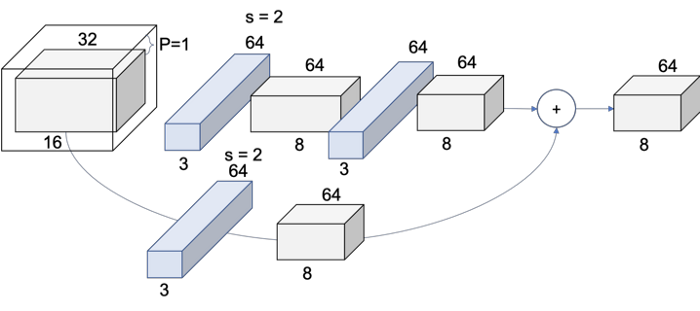
\includegraphics[scale=0.3]{img/layer3.png}
	\caption{Layer3 Residual Network}
	\label{fig:ResnetLayer3}
\end{figure}

\pagebreak

Sehingga formula akhir dari struktur Lightweight Residual Network dapat disimpulkan sebagai berikut \ref{fig:ResnetLayerFormula}

\begin{figure}[h!]
	\centering
	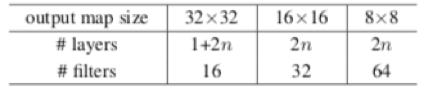
\includegraphics[scale=0.4]{img/ResNetFormula.png}
	\caption{Residual Network Formula}
	\label{fig:ResnetLayerFormula}
\end{figure}

Berikut merupakan perbandingan parameter Lightweight Residual Network dengan Residual Network

\begin{table}[h!]
	\begin{center}
		\begin{tabular}{|c|c|}
			\hline
			\textbf{Name} & \textbf{Parameters} \\ \hline
			ResNet 20 & 0.27M \\ \hline
			ResNet 32 & 0.46M \\ \hline
			ResNet 44 & 0.66M \\ \hline
			ResNet 56 & 0.85M \\ \hline
			ResNet 110 & 1.7M \\ \hline
			ResNet 50 & 23M \\ \hline
		\end{tabular}
	\end{center}
	\vspace{1ex}
	\caption{Parameter ResNet dibandingkan dengan Lightweight ResNet}
	\label{tabel:1}
\end{table}

\pagebreak

\section{Metode Pengujian}
\vspace{1ex}

\subsection{\textit{Precision}}
\vspace{1ex}
\textit{Precision} merupakan rasio dari prediksi jumlah total contoh positif yang benar diklasifikasikan dibagi dengan jumlah keseluruhan hasil yang diprediksi positif. Precision dapat melihat dari keseluruhan data, berapa persen yang diklasifikasikan secara benar.
\[Recall = \frac{TP}{(TP+FP)}\]

\subsection{\textit{Recall}}
\vspace{1ex}
Recall merupakan rasio dari jumlah total positif yang benar diklasifikasikan, dibagi dengan jumlah total contoh yang benar positif. Recall yang tinggi menunjukan bahwa kelas yang dikenali dengan benar banyak, atau False Negative yang didapatkan sedikit.
\[Recall = \frac{TP}{(TP+FN)}\]

\subsection{\textit{mean Average Precision} (mAP)}
\vspace{1ex}
\textit{mean Average Precision} (mAP) merupakan sebuah metrik akurasi yang didapatkan dari rata rata \textit{Average Precision}. Dimana Average Precision sendiri didapatkan dari perhitungan nilai presisi dan recall. mean Average Precision merupakan sebuah metrik evaluasi yang sangat baik dikarenakan melibatkan presisi dan recall. Dengan menggunakan mean Average Precision, sebuah angka dapat diterima untuk mengukur kinerja dari pendeteksian sebuah objek.

\[AP = \Sigma (recall_{n+1})-recall_n)\times precision_{interp}\times(recall_{n+1})\]

\subsection{\textit{Precision at n}}
\vspace{1ex}
\textit{Precision at n} merupakan sebuah metrik evaluasi yang didapatkan dari pengembalian informasi dalam bentuk daftar dengan ranking. Daftar ranking tersebut kemudian digunakan untuk melakukan penilaian dari akurasi model dengan cara melihat informasi ke-n paling atas yang dikembalikan. Rank-1 accuracy merupakan pengecekan berapa kali prediksi label sesuai dengan yang sebenarnya, sedangkan Rank-5 accuracy merupakan berapa kali prediksi label terdapat pada 5 prediksi paling atas.

\subsection{\textit{Re-Ranking}}
\vspace{1ex}
\textit{Re-Ranking} merupakan pengambilan \textit{K-Recriprocal Nearest Neighbor} yang mengambil citra serupa dengan citra \textit{query} yang diberikan. Hal ini dilakukan dengan adanya pengambilan jarak antara citra \textit{query} dengan citra yang terdapat pada \textit{gallery}.